\documentclass[a4paper,12pt,twoside]{memoir}

% Castellano
\usepackage[spanish,es-tabla]{babel}
\selectlanguage{spanish}
\usepackage[utf8]{inputenc}
\usepackage[T1]{fontenc}
\usepackage{lmodern} % scalable font
\usepackage{microtype}
\usepackage{placeins}

\RequirePackage{booktabs}
\RequirePackage[table]{xcolor}
\RequirePackage{xtab}
\RequirePackage{multirow}

% Links
\PassOptionsToPackage{hyphens}{url}\usepackage[colorlinks]{hyperref}
\hypersetup{
	allcolors = {red}
}

% Ecuaciones
\usepackage{amsmath}

% Rutas de fichero / paquete
\newcommand{\ruta}[1]{{\sffamily #1}}

% Párrafos
\nonzeroparskip

% Huérfanas y viudas
\widowpenalty100000
\clubpenalty100000

% Evitar solapes en el header
\nouppercaseheads

% Imagenes
\usepackage{graphicx}
\newcommand{\imagen}[2]{
	\begin{figure}[!h]
		\centering
		\includegraphics[width=0.9\textwidth]{#1}
		\caption{#2}\label{fig:#1}
	\end{figure}
	\FloatBarrier
}

\newcommand{\imagenflotante}[2]{
	\begin{figure}%[!h]
		\centering
		\includegraphics[width=0.9\textwidth]{#1}
		\caption{#2}\label{fig:#1}
	\end{figure}
}



% El comando \figura nos permite insertar figuras comodamente, y utilizando
% siempre el mismo formato. Los parametros son:
% 1 -> Porcentaje del ancho de página que ocupará la figura (de 0 a 1)
% 2 --> Fichero de la imagen
% 3 --> Texto a pie de imagen
% 4 --> Etiqueta (label) para referencias
% 5 --> Opciones que queramos pasarle al \includegraphics
% 6 --> Opciones de posicionamiento a pasarle a \begin{figure}
\newcommand{\figuraConPosicion}[6]{%
  \setlength{\anchoFloat}{#1\textwidth}%
  \addtolength{\anchoFloat}{-4\fboxsep}%
  \setlength{\anchoFigura}{\anchoFloat}%
  \begin{figure}[#6]
    \begin{center}%
      \Ovalbox{%
        \begin{minipage}{\anchoFloat}%
          \begin{center}%
            \includegraphics[width=\anchoFigura,#5]{#2}%
            \caption{#3}%
            \label{#4}%
          \end{center}%
        \end{minipage}
      }%
    \end{center}%
  \end{figure}%
}

%
% Comando para incluir imágenes en formato apaisado (sin marco).
\newcommand{\figuraApaisadaSinMarco}[5]{%
  \begin{figure}%
    \begin{center}%
    \includegraphics[angle=90,height=#1\textheight,#5]{#2}%
    \caption{#3}%
    \label{#4}%
    \end{center}%
  \end{figure}%
}
% Para las tablas
\newcommand{\otoprule}{\midrule [\heavyrulewidth]}
%
% Nuevo comando para tablas pequeñas (menos de una página).
\newcommand{\tablaSmall}[5]{%
 \begin{table}
  \begin{center}
   \rowcolors {2}{gray!35}{}
   \begin{tabular}{#2}
    \toprule
    #4
    \otoprule
    #5
    \bottomrule
   \end{tabular}
   \caption{#1}
   \label{tabla:#3}
  \end{center}
 \end{table}
}

%
%Para el float H de tablaSmallSinColores
\usepackage{float}

%
% Nuevo comando para tablas pequeñas (menos de una página).
\newcommand{\tablaSmallSinColores}[5]{%
 \begin{table}[H]
  \begin{center}
   \begin{tabular}{#2}
    \toprule
    #4
    \otoprule
    #5
    \bottomrule
   \end{tabular}
   \caption{#1}
   \label{tabla:#3}
  \end{center}
 \end{table}
}

\newcommand{\tablaApaisadaSmall}[5]{%
\begin{landscape}
  \begin{table}
   \begin{center}
    \rowcolors {2}{gray!35}{}
    \begin{tabular}{#2}
     \toprule
     #4
     \otoprule
     #5
     \bottomrule
    \end{tabular}
    \caption{#1}
    \label{tabla:#3}
   \end{center}
  \end{table}
\end{landscape}
}

%
% Nuevo comando para tablas grandes con cabecera y filas alternas coloreadas en gris.
\newcommand{\tabla}[6]{%
  \begin{center}
    \tablefirsthead{
      \toprule
      #5
      \otoprule
    }
    \tablehead{
      \multicolumn{#3}{l}{\small\sl continúa desde la página anterior}\\
      \toprule
      #5
      \otoprule
    }
    \tabletail{
      \hline
      \multicolumn{#3}{r}{\small\sl continúa en la página siguiente}\\
    }
    \tablelasttail{
      \hline
    }
    \bottomcaption{#1}
    \rowcolors {2}{gray!35}{}
    \begin{xtabular}{#2}
      #6
      \bottomrule
    \end{xtabular}
    \label{tabla:#4}
  \end{center}
}

%
% Nuevo comando para tablas grandes con cabecera.
\newcommand{\tablaSinColores}[6]{%
  \begin{center}
    \tablefirsthead{
      \toprule
      #5
      \otoprule
    }
    \tablehead{
      \multicolumn{#3}{l}{\small\sl continúa desde la página anterior}\\
      \toprule
      #5
      \otoprule
    }
    \tabletail{
      \hline
      \multicolumn{#3}{r}{\small\sl continúa en la página siguiente}\\
    }
    \tablelasttail{
      \hline
    }
    \bottomcaption{#1}
    \begin{xtabular}{#2}
      #6
      \bottomrule
    \end{xtabular}
    \label{tabla:#4}
  \end{center}
}

%
% Nuevo comando para tablas grandes sin cabecera.
\newcommand{\tablaSinCabecera}[5]{%
  \begin{center}
    \tablefirsthead{
      \toprule
    }
    \tablehead{
      \multicolumn{#3}{l}{\small\sl continúa desde la página anterior}\\
      \hline
    }
    \tabletail{
      \hline
      \multicolumn{#3}{r}{\small\sl continúa en la página siguiente}\\
    }
    \tablelasttail{
      \hline
    }
    \bottomcaption{#1}
  \begin{xtabular}{#2}
    #5
   \bottomrule
  \end{xtabular}
  \label{tabla:#4}
  \end{center}
}



\definecolor{cgoLight}{HTML}{EEEEEE}
\definecolor{cgoExtralight}{HTML}{FFFFFF}

%
% Nuevo comando para tablas grandes sin cabecera.
\newcommand{\tablaSinCabeceraConBandas}[5]{%
  \begin{center}
    \tablefirsthead{
      \toprule
    }
    \tablehead{
      \multicolumn{#3}{l}{\small\sl continúa desde la página anterior}\\
      \hline
    }
    \tabletail{
      \hline
      \multicolumn{#3}{r}{\small\sl continúa en la página siguiente}\\
    }
    \tablelasttail{
      \hline
    }
    \bottomcaption{#1}
    \rowcolors[]{1}{cgoExtralight}{cgoLight}

  \begin{xtabular}{#2}
    #5
   \bottomrule
  \end{xtabular}
  \label{tabla:#4}
  \end{center}
}




\graphicspath{ {./img/} }

% Capítulos
\chapterstyle{bianchi}
\newcommand{\capitulo}[2]{
	\setcounter{chapter}{#1}
	\setcounter{section}{0}
	\setcounter{figure}{0}
	\setcounter{table}{0}
	\chapter*{#2}
	\addcontentsline{toc}{chapter}{#2}
	\markboth{#2}{#2}
}

% Apéndices
\renewcommand{\appendixname}{Apéndice}
\renewcommand*\cftappendixname{\appendixname}

\newcommand{\apendice}[1]{
	%\renewcommand{\thechapter}{A}
	\chapter{#1}
}

\renewcommand*\cftappendixname{\appendixname\ }

% Formato de portada
\makeatletter
\usepackage{xcolor}
\newcommand{\tutor}[1]{\def\@tutor{#1}}
\newcommand{\course}[1]{\def\@course{#1}}
\definecolor{cpardoBox}{HTML}{E6E6FF}
\def\maketitle{
  \null
  \thispagestyle{empty}
  % Cabecera ----------------
\noindent
\includegraphics[width=\textwidth]{cabecera}\vspace{1cm}%
  \vfill
  % Título proyecto y escudo informática ----------------
  \colorbox{cpardoBox}{%
    \begin{minipage}{.8\textwidth}
      \vspace{.5cm}\Large
      \begin{center}
      \textbf{TFG del Grado en Ingeniería Informática}\vspace{.6cm}\\
      \textbf{\LARGE\@title{}}
      \end{center}
      \vspace{.2cm}
    \end{minipage}

  }%
  \hfill\begin{minipage}{.20\textwidth}
    
\includegraphics[width=\textwidth]{escudoInfor}
  \end{minipage}
  \vfill
  % Datos de alumno, curso y tutores ------------------
  \begin{center}%
  {%
    \noindent\LARGE
    Presentado por \@author{}\\ 
    en Universidad de Burgos --- \@date{}\\
    Tutores: \@tutor{}\\
  }%
  \end{center}%
  \null
  \cleardoublepage
  }
\makeatother


% Datos de portada
\title{Modelo de Propagación\\de Malware basado en\\Aprendizaje por refuerzo \\Documentación Técnica}
\author{Diego García Muñoz}
\tutor{Bruno Baruque Zanón y Roberto Carlos Casado Vara}
\date{\today}

\begin{document}

\maketitle



\cleardoublepage



%%%%%%%%%%%%%%%%%%%%%%%%%%%%%%%%%%%%%%%%%%%%%%%%%%%%%%%%%%%%%%%%%%%%%%%%%%%%%%%%%%%%%%%%



\frontmatter


\clearpage

% Indices
\tableofcontents

\clearpage

\listoffigures

\clearpage

\listoftables

\clearpage

\mainmatter

\appendix

\apendice{Plan de Proyecto Software}

\section{Introducción}
Este apartado está dedicado a la planificación del proyecto, ya fuese realizada antes de o durante el proyecto. Se cubre la planificación temporal del proyecto y sus tareas, además de los estudios de viabilidad, tanto económica como legal.


\section{Planificación temporal}

Para la planificación temporal del proyecto se decidió basarse en la metodología Scrum\cite{Scrum}, con varias modificaciones - como el no usar roles debido al número limitado de participantes, o el número reducido de reuniones - que se explican más exhaustivamente en el capítulo 4 de la memoria, Técnicas y Herramientas.

Por lo tanto, el trabajo se dividió en varias iteraciones o Sprints, al final de cada cual se tendría una versión mejorada del proyecto. Se decidió que la duración de estos Sprints sería de dos semanas, aunque los últimos se acortaron a Sprints de una semana para poder tener un seguimiento más granular de las tareas finales. Entre cada sprint se realizaba una reunión de seguimiento, revisando las tareas del anterior y planificando el siguiente Sprint. 

%Podría meter una planificación general, a grandes rasgos antes de empezar. Línea temporal o gráfico Gantt o algo

Al añadir tareas al tablero Scrum, se les indicaba una estimación del trabajo necesario y su dificultad mediante un valor numérico. Dichos valores no eran equivalentes a una medida real concreta, pues, aunque se podría cuantificar el esfuerzo mediante horas de trabajo, no se ha considerado una medición apropiada, pues no representa bien la posible dificultad de la tarea (una tarea podría llevar mucho tiempo pero consistir simplemente en acciones repetitivas y conocidas, requiriendo más esfuerzo que otra tarea mucho más pequeña pero que necesitase un análisis exhaustivo y cuidadoso de los pasos a realizar). Por lo tanto, los valores asignados a las tareas son una medida relativa, indicando que una tarea con una estimación de un 1 requerirá la mitad de esfuerzo que una tarea con una estimación de un 2, y 8 veces menos que una tarea con una estimación de un 8.

Estos valores luego se utilizaban a la hora de planificar cada Sprint, viendo el valor acumulado de las tareas realizadas en los sprints anteriores, y seleccionando tareas de una dificultad similar (excepto en casos que hubiese que acelerar el ritmo).

En cuanto al uso de GitHub y ZenHub para la ejecución de dicha planificación, se utilizaron los siguientes elementos:

\begin{itemize}
    \item \textbf{Issues (GitHub):} representan cada una de las tareas a realizar. Tenían diferentes campos personalizables:
    \begin{itemize}
        \item \textbf{Labels (GitHub):} permiten clasificar las tareas según categoría (documentación, investigación, funcionalidades...)
        \item \textbf{Estimate/Story Points (ZenHub):} representan una estimación del trabajo necesario para terminar la tarea, y la dificultad de ella. Es una medida relativa, como se ha explicado anteriormente.
    \end{itemize}
    \item \textbf{Sprints (ZenHub), Milestones (GitHub):} equivalentes a los Sprints del método Scrum, agrupan las tareas según la iteración en la que se van a realizar. Son equivalentes, pero se han utilizado ambos pues cada uno ofrecía funcionalidades ligeramente diferentes: los Milestones permitían incluir descripciones sobre los objetivos de la iteración, y los Sprints permitían que una misma tarea perteneciese a varias iteraciones, en caso de que no se pudiese terminar en un solo sprint.
    \item \textbf{Projects (ZenHub), Epics (GitHub):} agrupan las tareas en diferentes objetivos a largo plazo, y pueden incluir tareas de Sprints diferentes que estén relacionadas con el mismo objetivo. En general, los proyectos cubren un mayor plazo de tiempo que las épicas. 
    \item \textbf{Pipelines (ZenHub):} representan las diferentes fases de progreso para las tareas. Son las siguientes:
    \begin{itemize}
        \item \textbf{New Issues:} Tareas que aún no se han etiquetado ni realizado la estimación del esfuerzo.
        \item \textbf{Epics:} Épicas, al no formar parte de sprints en concreto se dejan separadas del resto.
        \item \textbf{Icebox:} Tareas que no son urgentes
        \item \textbf{Optional Product Backlog:} Tareas que, si se cuenta con el tiempo y recursos suficientes, sería recomendable hacer, pero no son necesarias para finalizar el proyecto.
        \item \textbf{Product Backlog:} Tareas que tienen que ser realizadas, pero no han sido asignadas a ningún Sprint.
        \item \textbf{Sprint Backlog:} Tareas asignadas al Sprint actual, en las cuales no se ha empezado a trabajar.
        \item \textbf{In Progress:} Tareas en las que se está trabajando en el momento.
        \item \textbf{Review/QA:} Tareas que han sido terminadas por el alumno, pendientes de revisión con los tutores en la reunión de final de Sprint. 
        \item \textbf{Closed:} Tareas revisadas por los tutores y que han sido corregidas por el alumno en caso de que fuese necesario. Se dan por terminadas permanentemente. 
    \end{itemize}
\end{itemize}

El conjunto de tareas del proyecto se puede encontrar en el siguiente enlace:
\url{https://github.com/dgm1003/TFG-RL-malware/issues}

Debido al uso que se le ha otorgado a los dos últimos pipelines, a la hora de visualizar los burndown charts es necesario indicar que aquellas tareas en la pipeline \textit{Review/QA} o posterior se tienen que considerar como completadas.

\imagen{BurndownChartConfig}{Configuración para la visualización correcta de gráficos Burndown}

\clearpage
El conjunto de Sprints que se realizaron fue el siguiente:

\subsection{Sprint 1: 24/02/2022 - 09/03/2022}

\imagen{Sprint1}{Burndown report del Sprint 1}

En este sprint se seleccionó los programas a utilizar durante el transcurso de las prácticas, y se empezó a aprender sobre los conceptos relacionados con el trabajo y las librerías que sería más posible que se acabasen utilizando.
También se comenzó el trabajo en la memoria del proyecto, empezando a definir los objetivos de dicho proyecto.

Se definieron demasiadas tareas, y subestimó el esfuerzo necesario para realizar algunas de ellas, por lo que solo se acabó completando algo más de la mitad de las tareas asignadas a este Sprint. Algunas, como la búsqueda de artículos relacionados, o la visualización de una presentación sobre el aprendizaje por refuerzo, se decidión aplazar por razones como la falta de conocimientos del alumno, o que la presentación no se había transmitido aún cuando finalizó el sprint.
\newpage

\subsection{Sprint 2: 10/03/2022 - 23/03/2022}

\imagen{Sprint2}{Burndown report del Sprint 2}

En este sprint se continuó con el aprendizaje, empezando a codificar con varios ejemplos y tutoriales, tanto de Reinforcement Learning como de Deep Reinforcement Leraning. Además, se redactaron en la memoria los conceptos teóricos vistos hasta el momento, y se definieron los diferentes elementos del problema a diseñar.
\newpage

\subsection{Sprint 3: 24/03/2022 - 06/04/2022}

\imagen{Sprint3}{Burndown report del Sprint 3}

En este sprint se continuó con el aprendizaje, leyendo más sobre los conceptos de aprendizaje por refuerzo y realizando más tutoriales con diferentes aspectos que parecieron interesantes de aprender para aplicar posteriormente en el proyecto. Además, se definió el problema de forma concreta, para así poder programar una versión inicial del algoritmo que resolviese dicho problema para una red muy simplificada.

Debido a un aumento de la carga de trabajo de las asignaturas universitarias, en este sprint se cubrieron menos Story Points, pero por lo demás transcurrió sin problemas.
\newpage

\subsection{Sprint 4: 07/04/2022 - 20/04/2022}

\imagen{Sprint4}{Burndown report del Sprint 4}

En este sprint se realizaron unos últimos tutoriales que se consideraron relevantes, cerrando así la fase de aprendizaje de conceptos básicos. Además, se definió el formato de las redes para el problema, y se utilizó la librería NetworkX para la generación de dichas redes, probando varios métodos hasta encontrar el adecuado.

Por otro lado, se fueron añadiendo características al código, como la separación en clases y funciones, el uso de función de recompensa, o la separación del algoritmo en entorno y agente. Si se consideraba que dichas características aportaban alguna ventaja, se usaba esa nueva versión del código como base para el resto de modificaciones, cosa que ocurrió con todos los cambios propuestos en este sprint.
\newpage

\subsection{Sprint 5: 21/04/2022 - 04/05/2022}

\imagen{Sprint5}{Burndown report del Sprint 5}

En este sprint se continuó con la programación del algoritmo de Tablas Q, dejando completadas la mayoría de las características necesarias. Por otro lado, se realizó una planificación a grandes rasgos de las tareas necesarias a realizar para completar el proyecto, al haberse pasado ya el punto intermedio del tiempo disponible para la realización del TFG en primera convocatoria. También, relacionado con este último punto, se definieron posibles ramas por las que ampliar el problema una vez terminado el algoritmo de Tablas Q
\newpage

\subsection{Sprint 6: 05/05/2022 - 18/05/2022}

\imagen{Sprint6}{Burndown report del Sprint 6}

En este sprint se completó el código del algoritmo de aprendizaje por tablas Q, con todas las funcionalidades que se consideraron necesarias para el trabajo. 

Por otro lado, se intentó crear la página web, para que los usuarios pudiesen introducir los datos del programa y visualizar los resultados obtenidos de una forma intuitiva, sin necesidad de entender la forma en la que estuviera programado el código. Además, se pretendía avanzar con la memoria, pero debido a la alta carga de trabajo académico en esas fechas, motivos personales, y subestimar la cantidad de trabajo necesario para esas tareas, no se pudo completar ninguna de ellas antes de finalizar el sprint.

\newpage

\subsection{Sprint 7: 20/05/2022 - 31/05/2022}

\imagen{Sprint7}{Burndown report del Sprint 7}

En este sprint se tuvo como objetivo crear el frontend completo de la página web, además de continuar con la redacción de la memoria, y ambas tareas fueron completadas. 

También se empezó a crear el backend, realizando modificaciones al código para que se pudiese adaptar a las necesidades de la página web, pero no se pretendió acabar esta tarea en el sprint.

\subsection{Sprint 8: 02/06/2022 - 15/06/2022}

En este sprint se intentó implementar el backend de la página web, además de continuar con la memoria, pero se contó con menos tiempo del esperado, y surgieron varios problemas a la hora de crear el backend que no fueron solucionados dentro del sprint, por lo que no se completó ninguna tarea.
\newpage

\subsection{Sprint 9: 16/06/2022 - 22/06/2022}

\imagen{Sprint9}{Burndown report del Sprint 9}

En este sprint se continuó con las tareas planificadas para el sprint 8, especialmente la resolución de problemas relacionados con la página web, cosa que no se consiguió. Aún así, se pudo avanzar en la memoria.

\subsection{Sprint 10: 23/06/2022 - 30/06/2022}

En este sprint se continuó con la implementación de la página web. Después de probar varias alternativas y considerar otras soluciones, se decidió dejar de utilizar \verb|docker-compose| y \verb|setuptools| para configurar las imágenes de docker, y pasar a una estructura más simple. Con este cambio se resolvieron algunos de los problemas, pero no todos. No se pudo completar ningún sprint, pero sí hubo progreso en el proyecto.
\newpage

\subsection{Sprint 11: 31/06/2022 - 06/07/2022}

\imagen{Sprint11}{Burndown report del Sprint 11}

En este sprint se continuó con la resolución de problemas de la página web. Se consiguió que funcionase la aplicación de Flask dentro del contenedor Docker, y el resto de problemas eran ya del propio código dentro del backend y del frontend, los cuales se decidieron abordar más adelante en agosto. Por otro lado, se definieron los casos de prueba para el estudio de valores óptimos que se pretendía realizar en el siguiente sprint.

\subsection{Sprint 12: 07/07/2022 - 22/07/2022}

\imagen{Sprint12}{Burndown report del Sprint 12}

En este sprint se realizó un estudio sobre qué valores de entrenamiento resultaban óptimos para obtener buenos resultados en un tiempo aceptable. Para ello se tuvo que adaptar el algoritmo para poder recoger estadísticas, y para poder ejecutar un gran número de experimentos de forma consecutiva. Una vez creada la versión del algoritmo para el estudio, se ejecutaron las pruebas, y analizaron los resultados. Se quiso también avanzar en la memoria, pero debido a ciertos motivos personales no hubo tiempo de realizar esa tarea.

\subsection{Sprint 13: 02/08/2022 - 08/08/2022}

\imagen{Sprint13}{Burndown report del Sprint 13}

En este sprint no se pudo trabajar bastantes de los días, por lo que se hizo menos trabajo que de normal, pero se pudo avanzar en la memoria, completando otro capítulo y medio.
\newpage

\subsection{Sprint 14: 09/08/2022 - 22/08/2022}

\imagen{Sprint14}{Burndown report del Sprint 14}

En este sprint se trabajó principalmente en la página web, solucionando los problemas que se encontraron en julio, y terminando todas las funcionalidades planificadas inicialmente. Además, se continuó con el trabajo en la memoria.

\subsection{Sprint 15: 23/08/2022 - 04/09/2022}

\imagen{Sprint15}{Burndown report del Sprint 15}

Este sprint se dedicó completamente a escribir la memoria, pretendiendo finalizar la mayoría de los capítulos y la totalidad de los anexos. Este objetivo fue cumplido casi en su totalidad, quedando solo un capítulo y algunos apartados por acabar en el siguiente sprint.

\subsection{Sprint 16: 05/09/2022 - 11/09/2022}

\imagen{Sprint16}{Burndown report del Sprint 16}

En este sprint se quiso acabar la memoria, y solucionar los problemas encontrados en el código en sprints anteriores, además de realizar pequeñas mejoras a la página web para conseguir una experiencia de usuario más satisfactoria. Además, se preparó el repositorio para la realización de pruebas unitarias en el siguiente sprint.

Sin embargo, hubo dificultades a la hora de encontrar trabajos relacionados, por lo que ese apartado se tuvo que aplazar al siguiente sprint.
\newpage

\subsection{Sprint 17: 12/09/2022 - 18/09/2022}

\imagen{Sprint17}{Burndown report del Sprint 17}

En este sprint se finalizó el trabajo. Por un lado, se acabó la memoria y realizaron las correcciones necesarias. Por otro lado, se crearon los tests unitarios para asegurar la calidad del código, y realizaron las refactorizaciones necesarias. Por último, se añadieron funcionalidades a la página web y se revisó el funcionamiento de todos los elementos del proyecto.


\section{Estudio de viabilidad}

\subsection{Viabilidad económica}
En este apartado se estudiará el impacto económico que tendría este proyecto en caso de que se desarrollase con fines comerciales. Se contará con los siguientes tipos de costes:

\subsubsection{Costes de personal}
El trabajo ha sido realizado por un desarrollador, a lo largo de un periodo de 8 meses, en el que se considera que ha trabajado a jornada completa. Suponiendo un salario medio de 1200 euros netos mensuales por un desarrollador, teniendo en cuenta que hay que sumarle el impuesto de IRPF y la cotización de la seguridad social, se obtendría el siguiente coste total:

\begin{table}[h]
\centering
\begin{tabular}{| l | r |}
\hline
Concepto & Coste \\ \hline
Salario mensual neto & 1200,00€ \\
Retención IRPF (14\%) & 331,69€ \\
Seguridad Social (35,35\%) & 837,51€ \\
Salario mensual bruto & 2369,20€ \\
Salario anual bruto (12 pagas)   & 28.430,40€ \\ \hline
\textbf{Total 8 meses} & \textbf{18.953,60€} \\ \hline
\end{tabular} 
\caption{Costes de personal}
\end{table}


Para el cálculo de la cotización a la seguridad social, se han considerado los siguientes valores \cite{seg-social:cotizacion}:
\begin{itemize}
    \item Contingencias comunes: 28,30\% (23,60\% de parte de la empresa y 4,70\% de parte del trabajador)
    \item Desempleo: 7,05\% (5,50\% de parte de la empresa y 1,55\% de parte del trabajador)
    \item \textbf{Total:} 35,35\%
\end{itemize}

Para el cálculo del IRPF, se ha considerado un 14\% de retención para salarios brutos anuales de entre 20.200,00 y 35.200,00 euros en Castilla y León \cite{jcyl:irpf}.


\subsubsection{Costes de equipamiento}

En cuanto al equipamiento, solamente se ha utilizado un ordenador portátil con un coste alrededor de los 900 euros. Se ha hecho uso de un sistema operativo Windows 10 -- además de una máquina virtual con Ubuntu para probar la página web -- pero se podía haber utilizado Ubuntu a lo largo de todo el proceso de desarrollo. Al ser Ubuntu un sistema operativo de código abierto y sin coste, no se tendrán en cuenta costes de sistema operativo. El resto del software utilizado en el transcurso del trabajo también ha sido gratuito. 

Considerando una amortización del 26\% anual para el portátil, y teniendo en cuenta que ha sido utilizado durante 8 meses, los costes de equipamiento serán:

\begin{table}[h]
\centering
\begin{tabular}{| l | r | r | r |}
\hline
Concepto & Coste & Amortización (1 mes) & Amortización (8 meses) \\ \hline
Portátil & 900€ & 19.50€ & 156€ \\ \hline
\textbf{Total} & \textbf{900€} & \textbf{19.50€} & \textbf{156€} \\ \hline
\end{tabular} 
\caption{Costes de equipamiento}
\end{table}


\subsubsection{Costes de página web}

Para la presentación del trabajo fin de grado, la página se ha diseñado para que los usuarios la ejecuten de manera local en un contenedor Docker. Si se desease pasar a un modelo comercial, sería necesario obtener un dominio web, como por ejemplo, un dominio .com.

En este caso, el precio del registro de un dominio .com tiene una media de 12,95€, obteniendo el dominio durante un año. Para poder usar el dominio en años posteriores, sería necesario pagar una renovación, también de 12,95€ anuales. En este apartado se considerarán solamente los costes iniciales.


\begin{table}[h]
\centering
\begin{tabular}{| l | r |}
\hline
Concepto & Coste \\ \hline
Registro dominio & 12,95€ \\ \hline
\textbf{Total} & \textbf{12,95€} \\ \hline
\end{tabular} 
\caption{Costes de página web}
\end{table}

Si se desease aumentar el rendimiento del algoritmo, reduciendo los tiempos de espera en redes con mayor número de nodos, habría que invertir en servidores, pero no se considerará esta situación en este apartado.



\subsubsection{Coste Total}

El coste total del proyecto será el siguiente:


\begin{table}[h]
\centering
\begin{tabular}{| l | r |}
\hline
Concepto & Coste \\ \hline
Costes de personal & 18.953,60€ \\
Costes de equipamiento & 156,00€ \\
Costes de página web & 12,95€ \\ \hline
\textbf{Total} & \textbf{19.122,55€} \\ \hline
\end{tabular} 
\caption{Coste total}
\end{table}


\subsubsection{Posibles fuentes de ingreso}

Existen varias posibilidades de obtener beneficios con el proyecto. El primero sería añadir banners de publicidad a los laterales de la página web, pero por sí solo la página necesitaría un tráfico muy elevado para ofrecer beneficios suficientes para hacer rentable el proyecto.

Una alternativa mas viable sería ofrecer suscripciones para diferentes niveles de cuentas de usuario. A los usuarios gratuitos se les impondría un límite sobre el tamaño de las redes que podrían configurar, y el número de veces que podrían realizar entrenamientos cada cierto tiempo. A los usuarios de pago se les levantarían esas restricciones, pudiendo tener diferentes niveles con más funcionalidades. 

Se podría hasta combinar ambas ideas, mostrando publicidad a los usuarios gratuitos pero no a los usuarios de pago, incentivando así a los usuarios a mejorar sus cuentas.

\subsection{Viabilidad legal}
En este apartado se hablará del proceso de selección de licencia del proyecto, además de posibles problemas que pudiesen surgir de un mal uso del programa, y cómo evitarlos o remediarlos.


\subsubsection{Licencia}
Las licencias de las dependencias y librerías utilizadas en el proyecto son:

\begin{table}[h]
\centering
\begin{tabularx}{\textwidth}{| l | >{\raggedright\arraybackslash}X | l |}
\hline
\textbf{Dependencia}  & \textbf{Descripción} & \textbf{Licencia} \\ \hline
Flask & Framework de desarrollo web & BSD-3\cite{licenses:Flask} \\ \hline
Numpy & Biblioteca de operaciones matemáticas y manejo de matrices & BSD-3\cite{licenses:Numpy} \\  \hline
NetworkX & Biblioteca para manejo y análisis de grafos & BSD-3\cite{licenses:NetworkX} \\  \hline
Matplotlib & Biblioteca para generación de gráficas & PSF\cite{licenses:Matplotlib} \\ \hline
Unittest & Framework para automatización de pruebas unitarias & PSF\cite{licenses:Unittest} \\ \hline
Random & Biblioteca propia de Python para la generación de números y secuencias aleatorias & PSF\cite{licenses:Python} \\ \hline
\end{tabularx}
\caption{Dependencias del proyecto y sus licencias}
\label{tab:licencias}
\end{table}

Correspondiendo ``BSD-3'' con la licencia Berkeley Software Distribution de 3 cláusulas\cite{licenses:BSD}, y ``PSF'' con la Python Software Foundation License\cite{licenses:PSF}. 

Considerando las licencias de las dependencias, habría que utilizar una licencia compatible en el proyecto. Se estuvo debatiendo entre una licencia BSD de 3 cláusulas o una licencia GPL 3.0, y se acabó escogiendo la primera, ya que permitiría, en un futuro, crear un software basado en este proyecto con una licencia más restrictiva, pudiendo dejar de ser código abierto. 

Esto puede ser positivo en este caso concreto, debido a que, si se desarrollase más el código, podría ser utilizado con fines maliciosos, por lo que sería necesario imponer restricciones sobre su uso, como se explica en el siguiente apartado.

Por lo tanto, la licencia escogida es una licencia \textbf{BSD de 3 cláusulas}, o \textbf{"New BSD"}. Esta licencia permite el uso, redistribución y modificación del código siempre que se mantenga el copyright, las condiciones y el aviso legal en dichas redistribuciones. Además, se necesitará autorización escrita de parte de los creadores y colaboradores del código original en caso de querer utilizar sus nombres para promocionar obras derivadas.

\subsubsection{Consideraciones legales}
Debido a las restricciones impuestas actualmente sobre las redes que representa, sería difícil utilizar el proyecto con fines maliciosos. Si se decidiese ampliar el proyecto y quitar esas restricciones, lo primero que habría que hacer sería dejar de tener el código fuente abierto al público, y cambiar la licencia del proyecto, pues si no cualquier persona podría copiarlo y utilizar una versión que no controlemos para hacer lo que desee. Por otro lado, habría que añadir un sistema de gestión de usuarios, con logs de uso por cada usuario, para poder regular posibles situaciones sospechosas.

También se podría enviar un correo a INCIBE\cite{Incibe} pidiéndoles un análisis del riesgo potencial de la aplicación, para poder recibir consejo sobre cuestiones como a qué tipos de organizaciones se podría ofrecer el servicio.
\apendice{Especificación de Requisitos}

\section{Introducción}
En este anexo se tratan los objetivos que se pretenden conseguir con este proyecto, los requisitos funcionales que se han fijado para cubrir dichos objetivos, y los casos de uso relacionados con ellos.

\section{Objetivos generales}

\begin{itemize}
    \item Realizar un algoritmo de aprendizaje por refuerzo que simule la propagación de un malware por una red de ordenadores, buscando la ruta óptima para llegar a un equipo objetivo.
    \item Crear una interfaz gráfica que permita a un usuario con conocimientos mínimos de programación configurar el algoritmo y utilizarlo.
\end{itemize}

\section{Catalogo de requisitos}
A continuación se listan los requisitos que se han definido para el proyecto.

\begin{description}
    \item[RF 1:] El usuario debe ser capaz de configurar y ejecutar un programa que permita entrenar un algoritmo de aprendizaje por refuerzo.
    \begin{description}
        \item[RF 1.1:] El programa deberá admitir un entorno sobre el que realizar el entrenamiento.
        \item[RF 1.2:] El usuario debe poder definir las tasas de aprendizaje y de descuento, y el número de episodios o iteraciones del entrenamiento.
        \item[RF 1.3:] Una vez introducidas las variables y definido el entorno, el usuario deberá ser capaz de entrenar el algoritmo.
        \item[RF 1.4:] El programa deberá poder encontrar la ruta óptima entre el punto inicial y la meta, una vez entrenado.
    \end{description}
    \item[RF 2:] El usuario debe ser capaz de generar y manejar un entorno que represente un malware en una red de ordenadores.
    \begin{description}
        \item[RF 2.1:] El entorno deberá contener una representación de la red de ordenadores, con información de qué dispositivos están infectados o son de alto riesgo.
        \item[RF 2.2:] El usuario debe poder definir las características de dicha red, que serán el número de dispositivos de la red, el porcentaje de dispositivos de alto riesgo, el dispositivo en el que empezará situado el malware, y el dispositivo objetivo que se quiere infectar. También podrá definir la seed utilizada en operaciones aleatorias, para poder reproducir pruebas de manera exacta.
        \item[RF 2.3:] El usuario debe poder seleccionar de entre varias redes predefinidas, con diferentes características, en vez de definir todos sus valores.
        \item[RF 2.4:] El entorno debe poder mostrar un listado de posibles acciones a realizar, dado su estado actual.
        \item[RF 2.5:] El usuario debe poder indicar al entorno que realice una acción, recibiendo información sobre el estado en el que se encuentra el entorno después de realizar dicha acción, la recompensa que ha obtenido, y si ha completado su objetivo o no.
        \item[RF 2.6:] El entorno debe ser capaz de mostrar una representación gráfica de su estado actual.
        \item[RF 2.7:] El usuario deberá poder reestablecer los valores del entorno a sus estados iniciales, para así poder reutilizar dicho entorno en otras situaciones.
    \end{description}
    \item[RF 3:] El usuario debe poder acceder a una página web que permita una fácil utilización del agente y entorno programados, sin necesidad de conocimientos de programación.
    \begin{description}
        \item[RF 3.1:] El usuario debe ser capaz de obtener una red de acuerdo a sus necesidades, ya sea introduciendo los valores de los parámetros concretos en un formulario, o seleccionando botones que correspondan a cada una de las redes predefinidas.
        \item[RF 3.2:] En caso de introducir manualmente los parámetros de la red, el usuario deberá poder seleccionar el nodo de origen y el nodo meta, después de ver una imagen de la red generada.
        \item[RF 3.3:] El usuario debe tener la posibilidad de definir mediante un formulario las tasas de aprendizaje y de descuento, y el número de episodios del entrenamiento, una vez terminada de configurar la red. 
        \item[RF 3.4:] Una vez definidos todos los parámetros, la página deberá pasar al entrenamiento del algoritmo, y una vez entrenado a la búsqueda de la ruta óptima desde el inicio hasta la meta, mostrando al final de este proceso la ruta y recompensa obtenida, además de una representación gráfica de la ruta tomada dentro de la red.
        \item[RF 3.5:] El usuario debe tener la opción de repetir la selección de red y el entrenamiento de agente tantas veces como desee.
    \end{description}
\end{description}
\newpage

\section{Especificación de requisitos}
\subsection{Diagrama de casos de uso}
A continuación se muestra el diagrama de casos de uso de la página web creada, pues es la parte del proyecto a la que accederá un usuario final, y contiene las funcionalidades del resto de componentes.

\imagen{DiagramaCasosDeUso}{Diagrama de casos de uso}

\subsection{Actores}
En el sistema actual solo existirá un actor, el usuario final. En caso de añadir algunas de las características comentadas en el estudio de viabilidad, sería necesario incluir como segundo actor un administrador de usuarios, con nuevos casos de uso asociados.

\newpage
\subsection{Especificación de casos de uso}
\begin{table}[h]
\centering
\begin{tabularx}{\textwidth}{| l | >{\raggedright\arraybackslash}X |}
\hline
\textbf{CU-01} & \textbf{Configurar red} \\ \hline
Descripción     & Permite al usuario configurar la red como desee. \\ \hline
Requisitos      & RF-2, RF-2.1, RF-2.2, RF-2.3, RF-2.6, RF-3, RF-3.1, RF-3.2 \\ \hline
Precondiciones  & La página web está disponible. \\ \hline
Secuencia       & 1. El usuario entra en la página web. \\
                & 2. El usuario selecciona si quiere introducir datos manualmente o seleccionar una red predefinida. \\
                & 3. El usuario completa los formularios de la opción que haya seleccionado. \\
                & 4. El usuario pulsa el botón ``Siguiente''. \\
                & 5. Si los datos son válidos, se crea una nueva red. \\ \hline
Postcondiciones & Una red con las especificaciones introducidas es creada. \\ \hline
Excepciones     & Se introducen los datos de forma incorrecta. \\ \hline
Importancia     & Alta \\ \hline
\end{tabularx}
\caption{Caso de uso 1: Configurar red}
\label{tab:CU-01}
\end{table}


\begin{table}[h]
\centering
\begin{tabularx}{\textwidth}{| l | >{\raggedright\arraybackslash}X |}
\hline
\textbf{CU-02}  & \textbf{Obtener ruta óptima} \\ \hline
Descripción     & Permite entrenar el algoritmo de aprendizaje por refuerzo y encontrar la ruta óptima del inicio a la meta. \\ \hline
Requisitos      & RF-1, RF-1.1, RF-1.2, RF-1.3, RF-1.4, RF-2, RF-2.4, RF-2.5, RF-2.6, RF-3, RF-3.3, RF-3.4, RF-3.5 \\ \hline
Precondiciones  & Se ha creado una red \\ \hline
Secuencia       & 1. El usuario introduce los datos del entrenamiento. \\
                & 2. El usuario pulsa el botón ``Entrenar''. \\
                & 3. Se crea un agente con la red existente. \\
                & 4. Se entrena el agente con los parámetros introducidos. \\
                & 5. Se pide al agente encontrar la ruta óptima. \\
                & 6. Se muestran los resultados. \\ \hline
Postcondiciones & Se muestra la ruta encontrada tanto en formato de texto como en representación gráfica. \\ \hline
Excepciones     & Los datos de entrenamiento introducidos son inválidos. \\ \hline
Importancia     & Alta \\ \hline
\end{tabularx}
\caption{Caso de uso 2: Obtener ruta óptima}
\label{tab:CU-02}
\end{table}


\begin{table}[h]
\centering
\begin{tabularx}{\textwidth}{| l | >{\raggedright\arraybackslash}X |}
\hline
\textbf{CU-03}  & \textbf{Introducir datos de la red} \\ \hline
Descripción     & Permite al usuario introducir los datos necesarios para generar una red. \\ \hline
Requisitos      & RF-2, RF-2.1, RF-2.2 \\ \hline
Precondiciones  & La página web está disponible. \\ \hline
Secuencia       & 1. El usuario selecciona el botón ``Introducir valores''. \\
                & 2. El usuario introduce el número de nodos (mayor que 0). \\
                & 3. Opcionalmente, el usuario introduce un valor numérico que sirva como seed para la generación aleatoria. \\
                & 4. El usuario introduce el porcentaje de nodos que serán de alto. riesgo (como un decimal entre 0 y 1) \\
                & 5. El usuario pulsa en ``Siguiente''. \\ \hline
Postcondiciones & Se ha creado una red sin nodo de inicio o meta. \\ \hline
Excepciones     & El número de nodos introducido es menor que 0, la seed introducida no es un valor numérico o el valor del porcentaje está por debajo de 0 o por encima de 1. \\ \hline
Importancia     & Alta \\ \hline
\end{tabularx}
\caption{Caso de uso 3: Introducir datos de la red}
\label{tab:CU-03}
\end{table}


\begin{table}[h]
\centering
\begin{tabularx}{\textwidth}{| l | >{\raggedright\arraybackslash}X |}
\hline
\textbf{CU-04}  & \textbf{Seleccionar inicio y meta} \\ \hline
Descripción     & Permite al usuario decidir qué nodos serán el origen y el objetivo del entrenamiento. \\ \hline
Requisitos      & RF-2, RF-2.1, RF-2.2, RF-2.6, RF-3, RF-3.2 \\ \hline
Precondiciones  & Se ha creado una red anteriormente por el método de introducir parámetros. \\ \hline
Secuencia       & 1. Se crea una representación gráfica de la red existente y se muestra al usuario. \\
                & 2. El usuario introduce el número del nodo inicial (no podrá ser menor a 0 o mayor o igual que el número de nodos de la red) \\
                & 3. El usuario introduce el número del nodo destino (no podrá ser menor a 0 o mayor o igual que el número de nodos de la red) \\
                & 4. El usuario pulsa en ``Siguiente''. \\
                & 5. Se actualiza la red con la nueva información. \\ \hline
Postcondiciones & La red actual pasa a tener nodos inicial y meta definidos. \\ \hline
Excepciones     & Los números de nodo inicial o meta introducidos son inválidos. \\ \hline
Importancia     & Alta \\ \hline
\end{tabularx}
\caption{Caso de uso 4: Seleccionar inicio y meta}
\label{tab:CU-04}
\end{table}


\begin{table}[h]
\centering
\begin{tabularx}{\textwidth}{| l | >{\raggedright\arraybackslash}X |}
\hline
\textbf{CU-05}  & \textbf{Seleccionar red predefinida} \\ \hline
Descripción     & Permite al usuario seleccionar de entre varias redes con diferentes configuraciones sin tener que introducir los datos manualmente. \\ \hline
Requisitos      & RF-2, RF-2.1, RF-2.3, RF-2.6 RF-3, RF-3.1 \\ \hline
Precondiciones  & La página web está disponible. \\ \hline
Secuencia       & 1. El usuario pulsa ``Seleccionar red predefinida''. \\
                & 2. Se muestran varios botones con información sobre las configuraciones de cada una de las redes, y una imagen de cada una. \\
                & 3. El usuario selecciona la red que desee utilizar. \\
                & 4. El usuario pulsa ``Siguiente''. \\
                & 5. Se crea la red con los parámetros seleccionados. \\ \hline
Postcondiciones & Una red con las especificaciones introducidas es creada. \\ \hline
Excepciones     & El usuario no selecciona ninguna red. \\ \hline
Importancia     & Media \\ \hline
\end{tabularx}
\caption{Caso de uso 5: Seleccionar red predefinida}
\label{tab:CU-05}
\end{table}


\begin{table}[h]
\centering
\begin{tabularx}{\textwidth}{| l | >{\raggedright\arraybackslash}X |}
\hline
\textbf{CU-06}  & \textbf{Configurar entrenamiento} \\ \hline
Descripción     & Permite al usuario definir los parámetros del entrenamiento. \\ \hline
Requisitos      & RF-1, RF-1.2, RF-3, RF-3.3 \\ \hline
Precondiciones  & Existe una red creada anteriormente. \\ \hline
Secuencia       & 1. El usuario introduce la tasa de aprendizaje (entre 0 y 1) \\
                & 2. El usuario introduce el factor de descuento (entre 0 y 1) \\
                & 3. El usuario introduce el número de episodios del entrenamiento (mayor que 0) \\
                & 4. El usuario pulsa el botón ``Entrenar''. \\
                & 5. Se guardan los datos del entrenamiento. \\ \hline
Postcondiciones & Los datos del entrenamiento han sido guardados. \\ \hline
Excepciones     & Se introducen valores inválidos en alguno de los tres campos. \\ \hline
Importancia     & Alta \\ \hline
\end{tabularx}
\caption{Caso de uso 6: Configurar entrenamiento}
\label{tab:CU-06}
\end{table}


\begin{table}[h]
\centering
\begin{tabularx}{\textwidth}{| l | >{\raggedright\arraybackslash}X |}
\hline
\textbf{CU-07}  & \textbf{Entrenar algoritmo y buscar ruta} \\ \hline
Descripción     & Permite al usuario obtener la ruta óptima entre el inicio y la meta después de un entrenamiento del algoritmo de aprendizaje por refuerzo. \\ \hline
Requisitos      & RF-1, RF-1.3, RF-1.4, RF-2, RF-2.4, RF-2.5, RF-3, RF-3.4 \\ \hline
Precondiciones  & Existe una red creada, y se tienen los parámetros del entrenamiento guardados. \\ \hline
Secuencia       & 1. Se crea un agente con la red existente. \\
                & 2. Se entrena el agente con los parámetros introducidos. \\
                & 3. Se pide al agente encontrar la ruta óptima. \\
                & 4. Se guarda la ruta encontrada y recompensa obtenida. \\ \hline
Postcondiciones & La ruta y recompensa obtenidas han sido guardadas. \\ \hline
Excepciones     & Ninguna \\ \hline
Importancia     & Alta \\ \hline
\end{tabularx}
\caption{Caso de uso 7: Entrenar algoritmo y buscar ruta}
\label{tab:CU-07}
\end{table}


\begin{table}[h]
\centering
\begin{tabularx}{\textwidth}{| l | >{\raggedright\arraybackslash}X |}
\hline
\textbf{CU-08}  & \textbf{Obtener resumen de resultados} \\ \hline
Descripción     & Permite al usuario visualizar los resultados del entrenamiento. \\ \hline
Requisitos      & RF-2, RF-2.6, RF-3, RF-3.4 \\ \hline
Precondiciones  & Se ha creado una red y se tiene una ruta desde el inicio hasta la meta. \\ \hline
Secuencia       & 1. Se genera una representación gráfica del recorrido de la ruta sobre la red. \\
                & 2. Se muestra la imagen generada junto a un resumen de los datos del entrenamiento y los resultados obtenidos. \\ \hline
Postcondiciones & Ninguna \\ \hline
Excepciones     & Ninguna \\ \hline
Importancia     & Alta \\ \hline
\end{tabularx}
\caption{Caso de uso 8: Obtener resumen de resultados}
\label{tab:CU-08}
\end{table}


\begin{table}[h]
\centering
\begin{tabularx}{\textwidth}{| l | >{\raggedright\arraybackslash}X |}
\hline
\textbf{CU-09}  & \textbf{Generar visualización del entorno} \\ \hline
Descripción     & Permite a la página web generar una visualización del estado en un momento concreto de la red de ordenadores. \\ \hline
Requisitos      & RF-2, RF-2.6 \\ \hline
Precondiciones  & Existe una red. \\ \hline
Secuencia       & 1. Se pide al entorno generar una representación gráfica de la red. \\
                & 2. En caso de haber una ruta, se pide al entorno priorizar los nodos de la ruta para que se vean más claramente que el resto. \\
                & 3. Se pide al entorno guardar la representación generada con un nombre concreto. \\ \hline
Postcondiciones & Se ha guardado una visualización de la red. \\ \hline
Excepciones     & Ninguna \\ \hline
Importancia     & Alta \\ \hline
\end{tabularx}
\caption{Caso de uso 9: Generar visualización del entorno}
\label{tab:CU-09}
\end{table}


\apendice{Especificación de diseño}

\section{Introducción}
En este apéndice se describen las consideraciones de diseño que se han tomado a la hora de crear un programa que cumpliese los requisitos tratados en el anexo anterior. Se explican las diferentes estructuras de datos del programa, su relación entre ellas, los procedimientos que realizan, y su distribución dentro de los paquetes del proyecto.

\section{Diseño de datos}
En esta sección se tratarán las consideraciones que se han tomado al representar y guardar los datos del algoritmo. Esto ha cambiado a lo largo de las diferentes versiones, pero solamente se va a considerar la versión final.

Para el almacenamiento de los datos en este proyecto, no se ha considerado necesaria una base de datos. Por lo tanto, todos los datos se almacenan en ficheros persistentes, o Estructuras de Datos dentro de los objetos que se van instanciando. Se explican a continuación estas estructuras.

\subsection{Diseño de datos en el algoritmo}
El algoritmo ha sido dividido en una clase de entorno y otra clase de agente. En los siguientes apartados se explicarán las diferentes estructuras de datos que forman parte de estas dos clases.

\subsubsection{Entorno}
Para la representación del entorno, se han utilizado los siguientes atributos de clase: 

\begin{itemize}
    \item \textbf{Red:} la red de ordenadores se representa mediante un grafo de NetworkX. Los nodos corresponden con los diferentes dispositivos de la red, y además, cada nodo contiene los siguientes atributos:
    \begin{itemize}
        \item \textbf{Riesgo:} un valor numérico indicando el riesgo de detección que tendrá el agente malware si pasa por ese nodo. Su valor mínimo es 1.
        \item \textbf{Infectado:} valor booleano, indica si el nodo está infectado o no.
        \item \textbf{Color:} este atributo lo tienen tanto los nodos como los enlaces. Permite mostrar información al renderizar el entorno, pues los nodos inicial y meta tendrán colores específicos, y aquellos nodos y conexiones por los que haya pasado el agente malware, o que haya infectado, pasarán a tener un color diferente.
    \end{itemize}
    \item \textbf{Número de nodos:} como indica su nombre, corresponde al número de nodos de la red. Es utilizado a la hora de generar el entorno, y ha sido designado como el número correspondiente a la acción de infectar el nodo actual (ya que no habrá nodos con ese número asignado a ellos). 
    \item \textbf{Meta:} valor numérico correspondiente al nodo objetivo.
    \item \textbf{Inicial:} valor numérico correspondiente al nodo origen. Es necesario guardarlo para poder resetear la red.
    \item \textbf{Estado actual:} valor numérico que registra en qué nodo se encuentra el malware en el instante de tiempo actual.
    \item \textbf{Tiempo límite:} número que indica el máximo de acciones que se pueden tomar antes de que se considere como finalizado el objetivo. Impide que un agente se quede tomando acciones sin llegar a la meta de forma infinita, pues de este modo, si no llega antes de un tiempo concreto, no se permiten más movimientos. Se ha definido como el doble del número de nodos, permitiendo al malware recorrer la red completa más de una vez hasta llegar a la meta. Es un valor muy pesimista, y se podría reducir, pero se ha dejado como está para tener una mayor seguridad de que se encuentra la ruta óptima.
\end{itemize}
Originalmente las recompensas para cada una de las acciones se guardaban en una matriz, pero más adelante se pasó a utilizar una función que calculaba la recompensa, para evitar problemas con redes muy grandes.

\subsubsection{Agente}

El agente contendrá dos elementos: Por un lado, tendrá una referencia al objeto del entorno sobre el cual se va a realizar el entrenamiento. Por otro lado, el agente también posee una \textbf{tabla Q}, correspondiente a una matriz en la que se guardan los valores de recompensa futura predecidos para cada par de estado-acción. Esta matriz tendrá un tamaño de $N*N+1$, siendo N el número de nodos de la red.

\subsection{Diseño de datos en la página web}

En el sitio web participa también una tercera clase, aquella que contiene los métodos para los endpoints de Flask. Esta clase utiliza variables de sesión para guardar los diferentes valores -- como los datos obtenidos en formularios -- sin perderlos al cambiar de página.

Sin embargo, uno de los elementos que se necesita que persistan entre las diferentes páginas del sitio web es el propio entorno, debido a la aleatoriedad con la que se genera. Para conseguir esta persistencia, ya que no se permitía guardar objetos de cualquier tipo en las variables de sesión en Flask, se optó por crear unos métodos que permitiesen transformar al entorno en un objeto JSON, compatible con las sesiones de Flask, y transformar al entorno de vuelta a su clase original a partir de un fichero JSON.

Por lo tanto, el entorno se transforma en un diccionario con las diferentes variables que lo forman, incluyendo la red, y a continuación se traduce a formato JSON. Debido a las limitaciones de tamaño que imponen algunos navegadores web sobre las variables de sesión, este método de almacenamiento del entorno tiene la consecuencia de que la red de ordenadores tendrá un límite de, aproximadamente, 150 dispositivos conectados. A efectos del proyecto actual no se ha considerado un problema, pues es un tamaño suficiente para probar el algoritmo, y si se desea ejecutarlo sobre redes más grandes se tiene acceso al código original exento de esta limitación, pero si se desea comercializar o publicar la página web, se deberá modificar este método de almacenamiento de datos.

Además, al generar representaciones gráficas del entorno, se ha añadido la opción de guardarlo como imagen, en unas carpetas concretas, con nombres predefinidos. De este modo, después de pedir al entorno dicha representación, el frontend es capaz de buscar en las rutas definidas y mostrar en la página web el estado del entorno en un momento determinado.

\subsection{Diagrama de clases}

La relación entre las tres clases explicadas anteriormente es la siguiente:

\imagen{DiagramaClases}{Diagrama de clases}




\section{Diseño procedimental}
En esta sección se explican los diferentes procedimientos que forman parte del proyecto, y los componentes que a su vez tienen esos procedimientos. 


Para poder hacer uso de un algoritmo de aprendizaje por refuerzo, es necesario tener un conjunto de estados, acciones y recompensas. En el proyecto actual, se han definido los siguientes:


\subsection{Acciones}
Las acciones que el agente podrá tomar serían:
\begin{itemize}
    \item Desplazarse a otro nodo conectado al actual
    \item Intentar infectar el nodo actual
\end{itemize}
    
De este modo, un agente puede infectar un nodo, moverse sin infectarlo, o moverse después de haberlo infectado.

En caso de pasar a un modelo estocástico, se indicó la posibilidad de añadir probabilidades a la acción de infectar, de modo que pudiese resultar en un equipo infectado o no dependiendo de lo bien defendido que estuviera dicho equipo. No se consideró para el problema actual.

\subsection{Estados}
Los dos valores más importantes de un estado son la posición del malware dentro de la red y la situación del nodo en el que se encuentra, que puede ser infectado o no infectado. Además de esos dos valores, también se tiene en cuenta el tiempo transcurrido desde que el malware se introdujo en el nodo inicial, y el estado de la red, es decir, el resto de nodos que han sido infectados. Por lo tanto, y junto con las acciones definidas anteriormentes, el entorno pasará de un estado a otro diferente cuando el malware se mueva a un nodo adyacente, o infecte el nodo actual, y esa acción se verá reflejada en el nuevo estado.

En caso de ampliar este problema a un proceso de decisión de Markov con un modelo estocástico, se indicó la posibilidad de añadir una tercera situación a los nodos: "detectado", que dificultaría el movimiento del malware, y podría ocurrir con diferentes probabilidades en cada nodo. Sin embargo, esto se consideró fuera del alcance del trabajo.

\subsection{Recompensas}

Se ha definido un conjunto de recompensas inicial, con el cual se considera que se puede llegar al nodo objetivo de una manera eficiente. Se le ha otorgado un valor numérico a cada una de las recompensas, pero esos valores indicando la relación entre los pesos de las diferentes recompensas, y pueden ser cambiados más adelante si se cree que será beneficioso para la eficiencia del algoritmo.
    
\begin{itemize}
    \item \textbf{(-1) a cada segundo que pasa sin haber llegado a la meta:} de este modo se promueve que el malware llegue a su destino lo más rápido posible.
    \item \textbf{(+999) al infectar el nodo objetivo:} consideramos que ha cumplido su meta entonces, por lo que le otorgamos una recompensa elevada.
    \item \textbf{(-5) al infectar un nodo diferente al objetivo:} esto aumentaría la probabilidad de que se detecte que está ocurriendo un ataque en la red, por lo que mientras se tenga un objetivo concreto no es recomendable.
    \item \textbf{(-3) en nodos hoja no objetivos:} tendrá que retroceder para seguir explorando, por lo que se consideran nodos con poco aporte de información, que es preferible evitar.
    \item \textbf{(-10) en nodos de alto riesgo:} aumentan la probabilidad de que los propietarios de la red detecten al malware, por lo que es preferible recorrer el mínimo número posible. 
    \item \textbf{(-111) al moverse de un nodo a otro si no están directamente conectados:} es algo que no debería ser posible, por lo que se penaliza gravemente.
\end{itemize}

Dado este conjunto de recompensas, se ha definido una función que, dado el estado actual y la acción que se desee tomar, calcula la recompensa obtenida.

\subsection{Procesos de entrenamiento y búsqueda de ruta}
Para el entrenamiento del algoritmo, se ha utilizado el método de Tablas Q con diferencia temporal, explicado más a fondo en el capítulo 3.1 de la memoria. 

El algoritmo mantiene una tabla Q, en la cual cada una de sus celdas corresponde a la recompensa futura (llamada valor) esperada al realizar una acción encontrándose en un estado concreto. Se ha optado por un entrenamiento por episodios, de modo que en cada episodio se iniciará el entorno con el malware en la posición de origen, e irá realizando acciones de manera aleatoria hasta llegar a su objetivo. Después de realizar cada acción actualizará la tabla Q, y una vez termine un episodio, reiniciará el entorno y comenzará el siguiente.

En cuanto a la búsqueda, partiendo del nodo de origen, el algoritmo tomará aquellas acciones que, según la tabla Q, prometan un mayor valor. De este modo, si el entrenamiento se ha realizado correctamente, encontrará la ruta óptima hasta el nodo objetivo.

\subsection{Diagramas de secuencia}
A continuación se muestran los diagramas de secuencia para los procesos de creación de la red introduciendo valores, entrenamiento del algoritmo y búsqueda de ruta óptima. Siempre ocurrirán los procesos en ese orden, pero se han separado para una mayor legibilidad.

No se muestra la secuencia de acciones para la creación de entorno mediante selección de modelos predefinidos, pues simplemente consiste en que el usuario pulsa el botón de la red que desea, y el Endpoint pide al constructor del entorno que genere la red seleccionada.

\imagen{DiagramaSecuenciaCreaRed}{Diagrama de secuencia del proceso de creación del entorno}

\imagen{DiagramaSecuenciaEntrenamiento}{Diagrama de secuencia del proceso de entrenamiento y búsqueda de ruta}

\section{Diseño arquitectónico}
En esta sección se explican las consideraciones tomadas al diseñar la arquitectura del proyecto.

\subsection{Arquitectura del algoritmo}
Para poder tener una mayor flexibilidad y posibilidad de reutilización del código, se ha decidido dividir el algoritmo en dos clases: una contiene el entorno completo y todas las operaciones relacionadas con modificar dicho entorno, y la otra contiene el agente de aprendizaje por refuerzo, que se encarga de realizar el entrenamiento y buscar rutas óptimas.

Para que haya compatibilidad entre entorno y agente, el entorno deberá ser una clase con las siguientes funciones:
\begin{itemize}
    \item \verb|step()|: dado el estado actual, realiza una acción. Deberá devolver el nuevo estado del entorno, la recompensa obtenida y un indicador de si ha completado o no su objetivo.
    \item \verb|render()|: genera una representación gráfica del entorno.
    \item \verb|reset()|: reinicia el entorno a sus valores iniciales.
    \item \verb|get_posibles_acciones()|: devuelve una lista con los números asociados a las diferentes acciones que es posible realizar dado un estado concreto.
\end{itemize}

Además, deberá contar con las variables \verb|inicial|, que indica el número del nodo en el que se empieza la ruta, y \verb|NNODOS|, que será equivalente al número de nodos de la red.

Al haber creado esta separación, se podrá utilizar una misma clase de agente para varios tipos de entornos o una misma clase de entorno en varios tipos de agente, con un mínimo de cambios.

Los tests unitarios se incluyeron en un paquete dentro del propio paquete del código fuente, para simplificar la importación del código.

\subsection{Arquitectura del sitio web}
Para la página web, se ha hecho uso de un diseño con separación entre backend y frontend. De este modo, el código del algoritmo se mantiene en el backend, y la representación de la página web en el frontend. Cuando el usuario introduce datos en un formulario o realiza una petición y es necesario hacer uso de las clases del backend, el frontend las llamará para obtener la información necesaria, sin tener que conocer su funcionamiento interno.

La estructura de paquetes es la siguiente:
\imagen{DiagramaPaquetes}{Diagrama de paquetes del sitio web}
\apendice{Documentación técnica de programación}

\section{Introducción}

En este anexo se explicarán todos aquellos aspectos relevantes para programadores, desde su estructura de directorios hasta las dependencias que tiene y que haya que instalar en ciertos casos, o el uso de los diferentes archivos que se encuentran en el repositorio.

\section{Estructura de directorios}

Los archivos del proyecto se distribuyen de la siguiente manera:

\begin{itemize}
    \item \verb|/| : contiene ficheros relativos a GitHub, como el ReadMe o la licencia.
    \item \verb|/Material de Tutoriales| : contiene aquellos archivos de código relacionados con los tutoriales y cursos realizados a lo largo del transcurso del proyecto.
    \item \verb|/memoria| : contiene los archivos \LaTeX y PDF de la memoria.
    \item \verb|/code| : carpeta en la que se encuentran todas aquellas subcarpetas que contienen el código del proyecto.
    \item \verb|/code/plainCode| : contiene todas las versiones por las que ha pasado el proyecto, para ejecutarse directamente en la consola sin necesidad de pasar por la página web, ofreciendo un mayor grado de libertad.
    \item \verb|/code/plainCode/tests| : contiene todos los tests unitarios correspondientes a cada una de las versiones del proyecto.
    \item \verb|/code/estudio| : contiene aquellos ficheros relacionados con el estudio de valores óptimos realizado durante el desarrollo del proyecto.
    \item \verb|/code/estudio/resultados_estudio_1| : en esta carpeta se fueron guardando las gráficas obtenidas al realizar el estudio mencionado anteriormente.
    \item \verb|/code/website| : esta carpeta contendrá todos los elementos relacionados con la página web, incluyendo un archivo Dockerfile utilizado a la hora de crear imágenes Docker, y scripts shell para crear una imagen y ejecutarla.
    \item \verb|/code/website/websiteCode| : en esta carpeta se encuentra un fichero con los requerimientos que es necesario instalar para que funcione la página web, además de la aplicación de Flask que creará la página web en sí.
    \item \verb|/code/website/websiteCode/backendContents| : contiene una versión del código del agente y entorno existente en \verb|/code/plainCode|, adaptada para su uso en la página web.
    \item \verb|/code/website/websiteCode/frontendContents| : contiene un fichero con las funciones a las que llaman los endpoints de la página web.  
    \item \verb|/code/website/websiteCode/frontendContents/static| : en esta carpeta se encuentra el fichero de estilo CSS
    \item \verb|/code/website/websiteCode/frontendContents/static/images| : aquí se guardan las imágenes que se utilizan en la página web.
    \item \verb|/code/website/websiteCode/frontendContents/templates| : contiene las plantillas Jinja con las que se generan las páginas HTML en el sitio web.
\end{itemize}


\section{Compilación, instalación y ejecución del proyecto}

Para poder utilizar el proyecto, una vez clonado el repositorio, será necesario instalar varias dependencias, en base a qué parte del proyecto se quiera ejecutar: la página web, los ficheros de código Python, o los archivos utilizados en los tutoriales.

\subsection{Instalaciones necesarias para la página web}

En el caso de la página web, solamente será necesario instalar Docker\cite{docker:install}. 

Una vez hecho esto se podrá proceder a construir la imagen necesaria y ejecutar un contenedor con ella, ya sea mediante los scripts de shell \verb|start.sh| y \verb|start.bat| proporcionados (para sistemas Linux y Windows respectivamente), o haciéndolo manualmente.

Un ejemplo del despliegue de la página web paso a paso consistiría en navegar a la carpeta \verb|websiteCode| en una terminal y ejecutar el siguiente comando para construir la imagen:

\begin{verbatim}
    docker build -t [nombre de la imagen] .
\end{verbatim}

Y a continuación ejecutar el siguiente comando para lanzar el contenedor:

\begin{verbatim}
    docker run -it -p 8080:8080 [nombre de la imagen]
\end{verbatim}

\subsubsection{Importar imagen Docker}

En vez de construirla desde cero, si se contiene un archivo .tar de la imagen, también se podrá importar con el siguiente comando:

\begin{verbatim}
    docker load --input [nombre archivo tar]
\end{verbatim}

Y a continuación lanzar el contenedor con el comando \verb|docker run| comentado anteriormente.

\subsection{Instalaciones necesarias para los ficheros de código}

Para poder ejecutar el código, será necesario tener Python\cite{python:install} instalado en el dispositivo. En el desarrollo se ha utilizado la versión 3.9, pero no utiliza funcionalidades específicas a esa versión, por lo que no habrá problema en utilizar otras diferentes.

Además de Python, se hace uso de varias librerías. Se podrán instalar mediante el fichero requirements.txt situado en\verb|/code/plainCode| o \verb|/code/website/websiteCode|, haciendo uso del siguiente comando:
\begin{verbatim}
    pip install -r requirements.txt
\end{verbatim}

Alternativamente, se pueden instalar manualmente con el comando \verb|pip install|. Las librerías necesarias son:
\begin{itemize}
    \item Flask\cite{Flask}, siendo recomendada la versión 2.0.1 al ser la utilizada en el desarrollo
    \item Numpy\cite{Numpy}
    \item NetworkX\cite{NetworkX}
    \item Matplotlib\cite{Matplotlib}
\end{itemize}

Para editar el código, se podrá utilizar cualquier editor de texto o entorno de desarrollo compatible con Python. En el desarrollo del proyecto se utilizó Visual Studio Code\cite{VSC} y, ocasionalmente, Spyder\cite{Spyder}.

\subsection{Instalaciones necesarias para el material de tutoriales}

En este caso, las dependencias varían con cada uno de los ficheros, pero incluyen todo lo mencionado en el apartado anterior, y además, las siguientes librerías:

\begin{itemize}
    \item Tensorflow
    \item gym
    \item keras
    \item keras-rl2
    \item pygame
    \item stable-baselines
\end{itemize}

Sin embargo, todas estas se utilizan solamente en ficheros \verb|.ipynb|, que realizarán la instalación automáticamente al ejecutarse, por lo que no será necesario instalar ninguna de ellas por separado. Lo que será necesario es un editor de archivos \verb|.ipynb|. No se requiere ninguno en concreto para la mayoría de archivos, aunque para su creación se utilizó Jupyter Notebook\cite{Jupyter} y Visual Studio Code. La única excepción es el archivo \verb|Gym_Env_Tutorial.ipynb|, que requiere de Google Colab\cite{Colab}.

\section{Manual del programador}

En este manual se tratarán aquellos temas que se consideran importantes para un programador que decida trabajar con el proyecto. Se hablará principalmente del propósito de los diferentes ficheros, su uso, y otras consideraciones relevantes que no se encuentren en otros capítulos de la memoria. 

Es importante destacar que todos los ficheros de código tienen comentarios explicando el funcionamiento, entradas y salidas de los diferentes métodos, y otra información relevante para el programador, de modo que no se tratarán esos aspectos dentro de este manual.

\subsection{Material de tutoriales}
Como se ha explicado anteriormente, en esta carpeta se encuentran los ficheros de código relacionados con los diferentes cursos y tutoriales que se han realizado durante el transcurso del proyecto. Por ello, y para evitar confusión, se incluye un enlace al tutorial correspondiente en el primer comentario de cada fichero.

Hay dos tipos de archivos en esta carpeta. Por un lado, archivos python (\verb|.py|) convencionales, y por otro lado archivos IPython Notebook (\verb|.ipynb|), los cuales se pueden editar y ejecutar utilizando Jupyter Notebook, pero también otros editores Python, como Visual Studio Code o PyCharm. Cabe destacar que el fichero \verb|Gym_Env_Tutorial.ipynb|, sin embargo, debe ejecutarse en Google Colab, al utilizar comandos exclusivos de ese entorno. 

Además, los ficheros cuyo nombre empieza con \verb|dqn_weights.h5f| forman parte del mismo tutorial que el archivo \verb|CartPole_Nicholas.ipynb|.

\subsection{Ficheros de código del algoritmo (alojados en la carpeta \texttt{plainCode})}
Aquí se encuentran todas las versiones por las que ha pasado el algoritmo. En general, el número de versión indica el orden en el que se fueron creando los ficheros, y los archivos con la misma versión están relacionados. Para ejecutarlos, habrá que ejecutar el archivo que se desee de entre los que tengan la nomenclatura \verb|algoritmo_v_X_X.py| o \verb|agente_Q_v_X_X.py|, pues son los que contienen el método \verb|main|, e importan otros de los ficheros.  

A continuación se ofrece una explicación de cada una de las versiones:

\begin{enumerate}
    \item \verb|algoritmo_v_0_0.py| : versión inicial del algoritmo, sin estructura de clases.
    \item \verb|algoritmo_v_0_1.py| : añade estructura de clases.
    \item \verb|algoritmo_v_0_2.py| : en vez de guardar la recompensa en una tabla, la obtiene mediante una función.
    \item \verb|pruebas_grafos.py| : pequeño programa con el que se probaron diferentes métodos de generación de redes de networkX, para decidir cuál utilizar
    \item \verb|algoritmo_v_0_3.py| : utiliza networkX para la representación de la red, en vez de una lista de tuplas correspondientes a las conexiones.
    \item \verb|algoritmo_v_0_4.py| y \verb|grafo_v_0_4.py| : se separa la red del propio algoritmo, haciendo independiente la representación de la red del propio aprendizaje. 
    \item \verb|agente_Q_v_1_0.py| y \verb|entorno_malware_v_1_0.py| : en vez de separar únicamente la red, se realiza una separación del entorno completo, que representa tanto a la red como al malware.
    \item \verb|agente_Q_v_1_1.py| y \verb|entorno_malware_v_1_0.py| : en vez de realizar un entrenamiento por iteraciones, se realiza un entrenamiento mediante episodios. El entorno no cambia, por lo que se utiliza el mismo.
    \item \verb|entorno_malware_v_1_2.py| : finaliza la funcionalidad de generar varias redes predefinidas en vez de introducir parámetros. Puede utilizarse en cualquiera de los agentes Q.
    \item \verb|agente_Q_v_2_0.py| y \verb|entorno_malware_v_2_0.py| : incluye funcionalidades añadidas primero a la página web, como la representación de nodos de riesgo en las gráficas y la posibilidad de redefinir qué nodos son de riesgo. Se considera la versión final del código fuente. 
\end{enumerate}

También existe otra versión del algoritmo, en la carpeta \verb|Estudio|, que ha sido modificada para recoger estadísticas del entrenamiento. El entorno no cambia, pero el agente, después de cada episodio, intenta buscar la ruta óptima, y recoge la puntuación obtenida. De ese modo se puede ver la progresión que ocurre durante el entrenamiento.

El archivo \verb|estudio_valores_1.py| contiene un conjunto de métodos que crean una lista de configuraciones, ejecutan el algoritmo con todas las posibles combinaciones, y guardan gráficas con los resultados. Se pueden crear nuevos estudios de valores fácilmente, duplicando el archivo y cambiando solamente los valores de la función de configurar experimentos y la carpeta en la que se guardan las gráficas.

\subsection{Sitio web}

En cuanto al código del sitio web, se han realizado varias modificaciones a los ficheros del agente y entorno, para poder adaptarlos a su uso en la web. Por un lado, al renderizar el entorno se ha añadido la opción de guardar la imagen obtenida en un directorio concreto. Por otro lado, el entorno tiene ahora dos nuevas funciones: \verb|to_json()| y \verb|from_json()|, que convierten a un objeto de entorno en un objeto tipo JSON, para así poder guardarlo como variable de sesión y hacer que persista entre unas páginas y otras. 

Un efecto secundario de este alcance es que, a partir de redes con 150 nodos aproximadamente, el tamaño del objeto JSON se vuelve muy grandes, y algunos navegadores no permiten cookies de este tamaño. A efectos del proyecto no es un problema, pues si se quiere utilizar el algoritmo con redes de un tamaño mayor se puede siempre utilizar el propio código, pero en caso de querer comercializarse o publicar el sitio web en internet será necesario enfocar la construcción de página web de un modo diferente.

En cuanto al frontend, se ha utilizado Flask que a su vez utiliza plantillas de Jinja2. El fichero \verb|frontendEndpoints.py| de la carpeta \verb|websiteCode| inicializa la aplicación Flask, configurando las rutas de las carpetas \verb|static| y \verb|templates|, y definiendo los endpoints del sitio web. estos endpoints llaman a los métodos correspondientes del fichero \verb|endpointMethods.py| de la carpeta \verb|frontendContents|, que se encargan de cargar las plantillas necesarias, recoger los datos de los formularios y comunicarse con el backend.

\subsection{Control de calidad}

En el repositorio se han integrado dos herramientas de control de calidad: Codacy y CodeClimate Quality.

Codacy ofrece una gran variedad de plantillas de control de calidad: Pylint, Bandit y Prospector para archivos Python, Hadolint para archivos Dockerfile, ShellCheck para archivos Shell, CSSLint y Stylelint para ficheros CSS. Esto le permite cubrir una gran variedad de problemas, desde errores de compilación, a posibles vulnerabilidades de seguridad a temas de estilo.

Por otro lado, los problemas que detecta Code Climate se centran especialmente en la facilidad de mantener el código, comprobando cosas como la longitud de los métodos, la dificultad de comprensión, o el número de argumentos que requieren. Además, solamente se analizan archivos de Python.

Se deshabilitaron algunos de los patrones, especialmente los relacionados con duplicación de código, pues debido a como se ha organizado el código, guardando todas las versiones por las que ha pasado, existe una gran cantidad de duplicación que es inevitable.

\section{Pruebas del sistema}

\subsection{Pruebas unitarias}
Junto a la versión en código plano se desarrollaron pruebas unitarias, para comprobar el correcto funcionamiento de los diferentes métodos del algoritmo. Se encuentran en el directorio \verb|/code/plainCode/tests|, y tienen la estructura de nombres \verb|test_X.py|, siendo X el nombre del archivo que se prueba en cada uno de ellos.

Para el desarrollo de dichas pruebas, se utilizó el framework Unittest, creando un archivo de pruebas por archivo de código fuente. Entre todos los ficheros de pruebas, se acabaron creando 59 casos de prueba. La mayoría corresponden con uno o varios métodos del código fuente, y contienen una breve explicación en los comentarios. 

La excepción son los casos de pruebas relacionados con los métodos de cálculo de recompensa. Debido a la alta complejidad de dichos métodos, se crearon varios casos de prueba para cada uno, dividiéndose en las siguientes comprobaciones:
\begin{itemize}
    \item Se comprueba que haya una penalización extrema para conexiones inexistentes en la red, y no exista esta penalización extrema para las conexiones que sí existen.
    \item Se comprueba que se tienen en cuenta los atributos de riesgo y falta de información (también llamado bajo valor) del nodo destino a la hora de calcular la recompensa.
    \item Se comprueba el cálculo correcto de las recompensas al infectar nodos no objetivo y objetivo
    \item Se comprueba que, al no moverse, la recompensa es negativa excepto si se está en el nodo objetivo y dicho nodo está infectado.
\end{itemize}

No se realizaron pruebas para el archivo \verb|algoritmo_v_0_0.py|, pues no cuenta con ninguna clase ni método.
\newpage
El conjunto de tests unitarios se puede ver a continuación:

\begin{figure}[!h]
	\centering
	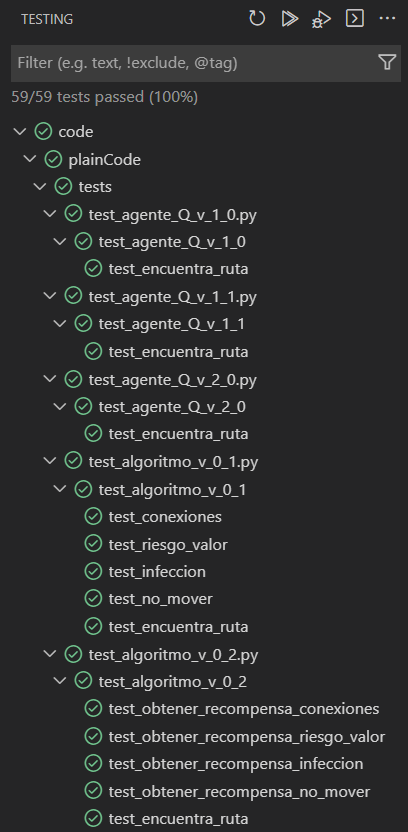
\includegraphics[width=0.6\textwidth]{tests1}
	\caption{Casos de prueba del proyecto. Parte 1}\label{fig:tests1}
\end{figure}
\begin{figure}[!h]
	\centering
	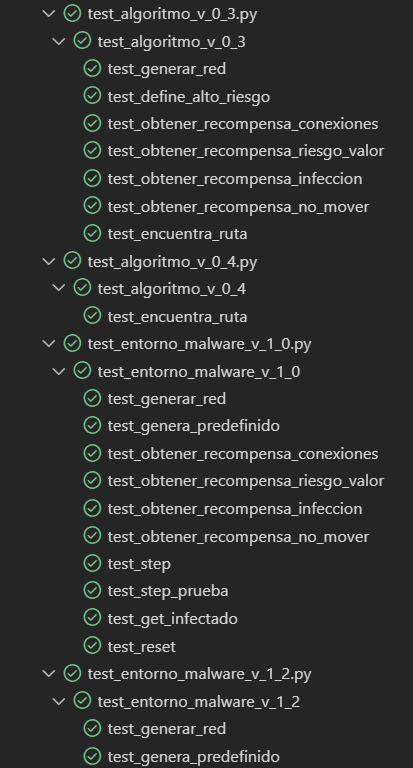
\includegraphics[width=0.6\textwidth]{tests2}
	\caption{Casos de prueba del proyecto. Parte 2}\label{fig:tests2}
\end{figure}
\begin{figure}[!h]
	\centering
	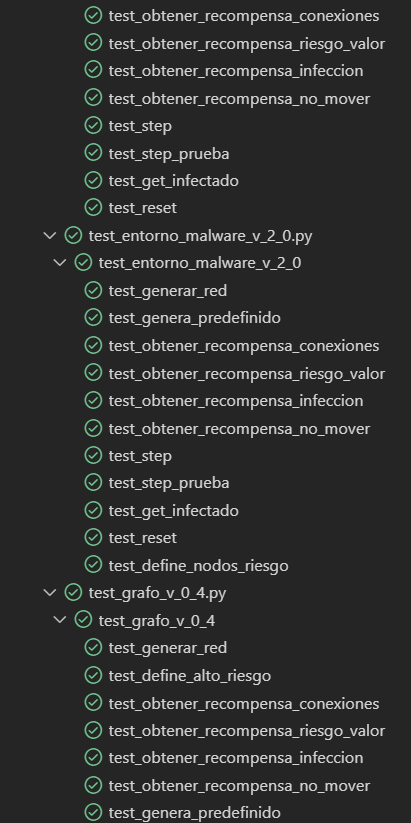
\includegraphics[width=0.6\textwidth]{tests3}
	\caption{Casos de prueba del proyecto. Parte 3}\label{fig:tests3}
\end{figure}
\FloatBarrier

\subsection{Estudio de valores de entrenamiento}
 
 Además de las pruebas unitarias, se decidió realizar un estudio de los valores de entrenamiento, para encontrar qué valores era recomendable asignar a cada variable para obtener resultados de manera consistentemente más rápida.
 
 \subsubsection{Realización del estudio}
 
 Se probó a modificar los siguientes parámetros:
 \begin{itemize}
     \item \textbf{Red de ordenadores:} se utilizaron la tercera, cuarta y quinta redes predefinidas en el código, formadas por 30, 300 y 3000 nodos respectivamente. Se hizo esto para cubrir diferentes situaciones y contextos en los cuales observar la influencia del resto de parámetros en el entrenamiento.
    \item \textbf{Tasa de aprendizaje (variable $\alpha$):} ya que es recomendable un valor entre 0 y 1, pero un valor de 0 resultaría en que no hubiese aprendizaje, se tomaron los valores con cifras decimales impares. Se pudo ver que un valor de 0.1 no aportaba mucha información relevante, así que se simplificó a los valores de 0.3, 0.5, 0.7 y 0,9.
    \item \textbf{Factor de descuento (variable $\gamma$):} también es un valor que debe estar entre 0 y 1, pero en este caso 0 es un número válido, por lo que se tomaron valores con cifras decimales pares, eliminando algunos que se consideraron similares a los demás para evitar una cantidad desorbitada de experimentos. Se acabaron usando los valores 0.2, 0.4, 0.8 y 1.
    \item \textbf{Número de episodios:} debido a los diferentes tamaños de las redes, se necesitaban diferentes números de episodios para realizar entrenamientos satisfactorios. Por ello, se definieron los valores de 5, 50, 100 y 200, pues con 200 se era capaz de entrenar la el entorno más grande de los seleccionados sin problema, y así se cubría un gran rango de valores. Sin embargo, estos números de episodios tan elevados no tenían sentido en redes pequeñas, pues se encontraba la ruta óptima mucho antes, por lo que no ofrecían información estos experimentos, y se decidieron eliminar. 
 \end{itemize}
\newpage

 \begin{table}[h]
\centering
\begin{tabular}{|l|cccc|}
\hline
\textbf{Parámetro}  & \multicolumn{4}{c|}{\textbf{Valores}}    \\ \hline
Nodos de la red     & 30      & \multicolumn{2}{c}{300} & 3000 \\ \hline
Tasa de aprendizaje & 0,3     & 0,5     & 0,7           & 0,9  \\ \hline
Factor de descuento & 0,2     & 0,4     & 0,8           & 1    \\ \hline
Número de episodios & 5       & 50      & 100           & 200  \\ \hline
\end{tabular}
\caption{Valores de los parámetros de los experimentos}
\label{tab:valores-experimentos}
\end{table}


 Se realizó un experimento con cada posible combinación de parámetros. Como se explica en el apartado de Aspectos Relevantes en la memoria principal, estos experimentos consistían en la realización del entrenamiento del agente con dichos parámetros, con la particularidad de que al final de cada episodio se realizaba una búsqueda de la ruta y se registraba su puntuación, pudiendo ver así el progreso del aprendizaje.
 
\imagen{graficaExperimento}{Ejemplo de gráfica obtenida al realizar uno de los experimentos}
 
 Debido a las recompensas definidas para el Proceso de Decisión de Markov del proyecto, cuando el algoritmo no encontraba la ruta obtenía una recompensa negativa de una magnitud considerablemente mayor a la recompensa positiva obtenida al encontrar una ruta óptima. Por lo tanto, en el eje Y las gráficas se obtiene una escala muy grande, que hace difícil visualizar la evolución a partir del momento en el cual se encuentra una ruta hasta el objetivo, pero muestra muy claramente el momento en el que el algoritmo encuentra esa ruta. Este segundo valor es el que se comparó en el estudio.
 
 \subsubsection{Resultados obtenidos}
 Los resultados fueron los siguientes:

\begin{itemize}
    \item En cuanto al \textbf{número de episodios}, con 50 es generalmente suficiente para redes de hasta 300 nodos, pero a partir de esos valores, aunque en general puede seguir ocurriendo que se encuentre la ruta pronto, es cada vez más posible que no se encuentre a tiempo, por lo que se recomienda aumentar el número de episodios, por ejemplo a 100.
    
    \imagen{estudioEpisodios}{Ejemplos del número de episodios que se tarda en converger dependiendo del tamaño de la red}
    
    \item Se descubrió que, generalmente, la \textbf{tasa de aprendizaje} acelera el proceso de entrenamiento a medida que va aumentando. Sin embargo, con redes grandes, valores muy elevados resultaron en que el algoritmo tardase más en encontrar una ruta. Por ello, se decidió recomendar un $\alpha$ de 0,9 en redes de hasta 300 nodos, y valores ligeramente menores a partir de entonces.
    
    \imagen{estudioAlpha}{Ejemplos de la influencia de la tasa de aprendizaje en la velocidad de convergencia}
    
    \item Por otro lado, se observó como la \textbf{tasa de descuento} acabó influyendo con menos frecuencia en los resultados. Sin embargo, se pudo ver como la mayoría de las veces, a valores mayores, el entrenamiento encontraba resultados ligeramente antes que en los otros experimentos, pero cuando se acercaba a valores de 1, volvía a aumentar el tiempo hasta la convergencia. Por lo tanto, se recomendó utilizar un $\gamma$ de 0,8 aunque, como se dice antes, tiene menor influencia sobre los resultados que la tasa de aprendizaje.
    
    \imagen{estudioGamma}{Ejemplos de la influencia del factor de descuento en la velocidad de convergencia}
    
\end{itemize}
\apendice{Documentación de usuario}

\section{Introducción}
En este anexo se explicará los requisitos necesarios para ejecutar la aplicación y el proceso de instalación y puesta en marcha. También se incluye una guía para orientar al usuario por las diferentes páginas.

\section{Requisitos de usuario}
Los requisitos para poder utilizar la aplicación son los siguientes:

\begin{itemize}
    \item Tener un sistema operativo compatible con Docker\cite{docker:install}, como Ubuntu, o Windows con la versión Docker Desktop.
    \item Tener Docker instalado en dicho sistema operativo.
    \item Contar con un navegador de internet.
\end{itemize}


\section{Instalación y ejecución}

Para instalar y levantar la página web del proyecto, se deberán seguir los siguientes pasos:

\begin{enumerate}
    \item Descargar el repositorio del proyecto
    \item Abrir una ventana de la terminal
    \item Dirigirse a la carpeta del proyecto, y a continuación navegar hasta la carpeta \verb|/code/website| (por ejemplo, en Ubuntu y Windows se podrá navegar con el comando \verb|cd [nombre de directorio]| )
    \item Escribir \verb|./start.sh| si se está en un sistema operativo Ubuntu, o \verb|start.bat| si se está en un sistema operativo Windows.
    
    Este comando ejecutará el fichero del nombre correspondiente, que instalará la imagen Docker del proyecto, en caso de que no haya sido instalada anteriormente, y a continuación ejecutará un contenedor de dicha imagen. Si se está utilizando un sistema operativo que no soporte esas extensiones de fichero, en vez del último paso se puede abrir cualquiera de los ficheros en un editor de texto y copiar los dos comandos existentes dentro de la terminal.
    
    Deberán aparecer una o varias direcciones http por pantalla:
    
    \imagen{FlaskRunning}{Ejemplo de la aplicación en ejecución}
    
    \item introducir en el navegador web una de las url mostradas en el paso anterior
\end{enumerate}

Si se desea dejar de utilizar el programa, se puede detener con Ctrl+C.

\subsection{Importación de imagen Docker si se dispone de ella}

En caso de tener acceso a la imagen Docker en formato .tar, se podrá importar al equipo, evitando el proceso de instalación. Habrá que seguir los siguientes pasos:

\begin{enumerate}
    \item Descargar el repositorio del proyecto
    \item Abrir una ventana de la terminal
    \item Dirigirse a la carpeta que contenga la imagen (por ejemplo, en Ubuntu y Windows se podrá navegar con el comando\\ \verb|cd [nombre de directorio]| )
    \item Escribir el siguiente comando para importar la imagen docker:
    
        \verb|docker load --input [nombre del archivo .tar]|
    \item Escribir el siguiente comando para ejecutar el contenedor docker e iniciar la página web:
    
        \verb|docker run -it -p 8080:8080 [nombre de la imagen]|
    
    A partir de aquí, el procedimiento es idéntico a la otra alternativa. Deberán aparecer una o varias direcciones http por pantalla.
    
    \item introducir en el navegador web una de las url mostradas en el paso anterior
\end{enumerate}

Si se desea dejar de utilizar el programa, se puede detener con Ctrl+C.

\section{Manual del usuario}

A continuación se explicarán paso a paso las diferentes funcionalidades de la aplicación.

\subsection{Generación de red}

Al entrar en la página web, además de una breve descripción de la página, se le presenta al usuario con dos opciones para generar su red, brevemente explicadas:

\imagen{manualusuario1}{Página inicial, seleccionando opción de introducir datos de red}
\imagen{manualusuario2}{Página inicial, seleccionando opción de elegir red predefinida}

\subsubsection{Generación de red introduciendo valores}

Al seleccionar la primera opción, nos redirigirá al siguiente formulario:

\imagen{manualusuario3}{Página de introducir datos de la red}

En ella, nos pedirá los siguientes valores:

\begin{itemize}
    \item \underline{Número de nodos:} corresponde al número de dispositivos que tendrá la red. Es un campo obligatorio.
    \item \underline{Semilla (opcional):} las redes se generan de forma aleatoria, pero para poder controlar esta aleatoriedad se puede utilizar una semilla (también conocida como seed). Mientras dos redes tengan el resto de datos iguales, si tienen semillas diferentes sus generaciones serán diferentes, pero si su seed es la misma, serán idénticas, lo cual será muy útil si se quiere reproducir una ejecución varias veces con las mismas condiciones. En nuestro caso la semilla consistirá en un valor numérico.
    \item \underline{Porcentaje de nodos de alto riesgo (entre 0 y 1):} dentro de la red existen nodos que se considera que son de alto riesgo, pues sus defensas serán mayores y la probabilidad de detección será más alta. Por ello, el algoritmo intentará evitar esos nodos. En la generación de la red, se seleccionarán de forma aleatoria, y en este campo se puede definir la probabilidad de que cada nodo sea asignado un alto riesgo. Por defecto tiene un valor de 0,25, es decir, cada nodo tendrá un 25\% de probabilidades de ser de alto riesgo.
\end{itemize}

Una vez rellenados los campos, habrá que pulsar en el botón ``Siguiente'', y se pasará a la selección de nodo inicial y final:

\imagen{manualusuario4}{Página de selección de origen y meta}

Aparecerá una imagen, que mostrará los nodos de la red y todas las conexiones entre ellos. Cada nodo tendrá un identificador numérico. Debajo de la imagen, habrá dos campos, pidiendo el nodo inicial y objetivo respectivamente. En estos campos se tendrá que escribir el número identificativo de los nodos que se desee. 

También se podrá ver un tercer campo, opcional, para redefinir los nodos de riesgo. Se puede introducir una lista de números de nodos, separados por espacios, y estos nodos pasarán a ser los nuevos nodos de alto riesgo que el algoritmo deberá evitar a ser posible. Los antiguos nodos definidos como de alto riesgo volverán a ser nodos de riesgo normal, a no ser que se hayan incluido en la nueva lista.

Una vez se hayan rellenado los campos deseados, se deberá pulsar en el botón ``Siguiente'' para finalizar la configuración de la red.

\subsubsection{Generación de red seleccionando red predefinida}

Si se seleccionó la segunda opción en vez de la primera en la página principal, llevará a una página diferente, en la que aparecerá información sobre varios grafos, junto a una imagen representativa de cada uno.

\imagen{manualusuario5}{Página de selección de redes predefinidas}

El usuario simplemente tendrá que seleccionar la red que le interese y pulsar ``Siguiente'', sin tener que introducir ningún otro tipo de información.

\newpage
\subsection{Entrenamiento}

Independientemente de como se haya decidido generar la red, el sitio web acabará dirigiendo al usuario a la siguiente página:

\imagen{manualusuario6}{Página de configuración del entrenamiento}

En esta página se requieren los siguientes datos:

\begin{itemize}
    \item \underline{Tasa de aprendizaje (alpha):} esta tasa, entre 0 y 1, indicará la importancia que tendrán los movimientos nuevos durante el entrenamiento sobre el agente de aprendizaje por refuerzo. A tasas de aprendizaje muy bajas, su comportamiento se modificará a una velocidad más lenta, y tardará más en encontrar la solución óptima. Con tasas de aprendizaje muy elevadas, dará mucha importancia a los resultados de cada movimiento que realice, modificando su comportamiento muy rápidamente, y pudiendo pasarse por alto la solución óptima. Es por esto que es muy importante encontrar una tasa de aprendizaje apropiada a cada situación.
    
    \item \underline{Factor de descuento (gamma):} este valor, también entre 0 y 1, representa la importancia que le dará el agente a las posibles recompensas futuras. A valores muy altos, buscará maximizar las recompensas a corto plazo, y a valores muy bajos, intentará maximizar las recompensas a largo plazo. La recompensa a largo plazo es siempre una estimación, pues el agente no puede saber con certeza el valor exacto, por lo que puede darse la situación en la que, a factores de descuento muy bajos, el agente tome decisiones que aporten menor beneficio a corto plazo, esperando recompensas mayores en el futuro que no lleguen a materializarse. Por ello también es importante utilizar valores apropiados, y no muy extremos.
    
    \item \underline{Número de episodios del entrenamiento:} representa la duración del entrenamiento. A valores más altos tardará más tiempo en terminar, pero a valores muy bajos es posible que no le dé tiempo a encontrar la ruta óptima.
\end{itemize}

Una vez completados los campos, al pulsar en el botón ``Entrenar y obtener ruta'', la página hará exactamente eso, entrenará el agente de aprendizaje por refuerzo, y le pedirá buscar la ruta óptima entre el origen y el objetivo. Al finalizar, mostrará la página de resultados:

\imagen{manualusuario7}{Página de resultados}

En ella se podrá ver la ruta obtenida, tanto en la imagen como en el texto debajo de ella, además de la recompensa final, y un resumen de los datos de entrenamiento para facilitar la repetición del experimento.


\subsection{Repetición del proceso}

Si se quisiera volver a empezar todo el proceso, ya sea por algún error al introducir los datos, o para realizar otro entrenamiento después de haber finalizado uno, simplemente bastará con pulsar el botón de ``Volver a inicio'' presente en todas las páginas del sitio web.


\bibliographystyle{plain}
\bibliography{bibliografiaAnexos}

\end{document}
